\documentclass[../../main.tex]{subfiles}

\begin{document}

\begin{sloppypar}
Die Analyse der Interviews stützt sich auf das von \citeauthor{mayring_qualitative_2015} (\citeyear{mayring_qualitative_2015}) beschriebene Verfahren der qualitativen Inhaltsanalyse eines Ausgangsmaterials mittels Zusammenfassung / Kategorisierung und der anschliessenden Reduktion durch Paraphrasierung mit anschliessender Bündelung, Selektion und erneuter Bündelung / Konstruktion. \citeauthor{mayring_qualitative_2015} sagt zur zusammenfassenden Inhaltsanalyse, resp. zur Kategorisierung:

\begin{quote}
"`Die zusammenfassende Inhaltsanalyse [\dots] versucht alles Material zu berücksichtigen und systematisch auf das Wesentliche zu reduzieren."' (\cite{mayring_qualitative_2015}, S. 68).
\end{quote}

\begin{quote}
"`Eine induktive Kategoriendefinition hingegen leitet die Kategorien direkt aus dem Material in einem Verallgemeinerungsprozess ab, ohne sich auf vorab formulierte Theorienkonzepte zu beziehen"' (\cite{mayring_qualitative_2015}, S. 85).
\end{quote}

Das Ausgangsmaterial (hier: Audioaufnahmen) wird zuerst paraphrasiert. Anschliessend wird es durch Generalisierung, Selektion/Streichung (Auslassung) weiter reduziert und durch Bündelung gleicher oder ähnlicher Aussagen, resp. durch die Konstruktion und Integration mehrerer Aussagen zum gleichen Gegenstand schliesslich in eine neue Aussage überführt (vgl. \citeauthor{mayring_qualitative_2015} \citeyear{mayring_qualitative_2015}, S. 71 f.).

Die nachfolgende Abbildung illustriert dieses Verfahren anhand von zwei Durchgängen durch die Vorgänge Selektion/Streichung und Bündelung/Konstruktion.

%% -
%% - keep this block together!!!!!!!!!!!!!!
%% - --------------------------------------
%% -
\addtocounter{figure}{1}
\begin{figure}[H]
 \centering
 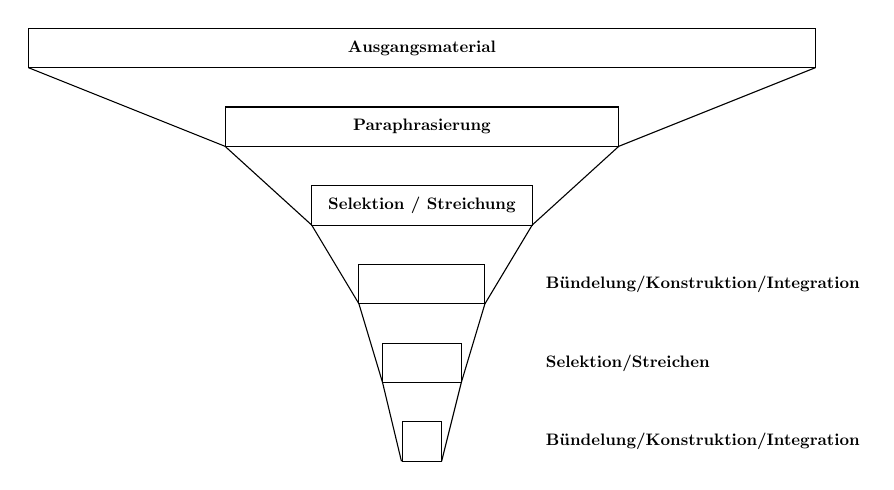
\begin{tikzpicture}

\draw[black, thin] (0,8) rectangle (10,7.5);
\node[draw,scale=0.6,shape=rectangle,draw=none,font=\bf] at (5,7.75) {Ausgangsmaterial};

\draw[black, thin] (2.5,7) rectangle (7.5,6.5);
\node[draw,scale=0.6,shape=rectangle,draw=none,font=\bf] at (5,6.75) {Paraphrasierung};

\draw[black, thin] (3.6,6) rectangle (6.4,5.5);
\node[draw,scale=0.6,shape=rectangle,draw=none,font=\bf] at (5,5.75) {Selektion / Streichung};

\draw[black, thin] (4.2,5) rectangle (5.8,4.5);
\node[draw,scale=0.6,shape=rectangle,anchor=west,draw=none,font=\bf] at (6.5,4.75) {Bündelung/Konstruktion/Integration};

\draw[black, thin] (4.5,4) rectangle (5.5,3.5);
\node[draw,scale=0.6,shape=rectangle,anchor=west,draw=none,font=\bf] at (6.5,3.75) {Selektion/Streichen};

\draw[black, thin] (4.75,3) rectangle (5.25,2.5);
\node[draw,scale=0.6,shape=rectangle,anchor=west,draw=none,font=\bf] at (6.5,2.75) {Bündelung/Konstruktion/Integration};

\draw[black, thin] (0,7.5) -- (2.5,6.5) -- (3.6,5.5) -- (4.2,4.5) -- (4.5,3.5) -- (4.74,2.5);
\draw[black, thin] (10,7.5) -- (7.5,6.5) -- (6.4,5.5) -- (5.8,4.5) -- (5.5,3.5) -- (5.25,2.5);

\end{tikzpicture}
 \caption*{Abbildung \thefigure: Materialreduzierung durch die Zusammenfassung; aus: \citeauthor{mayring_qualitative_2015} (\citeyear{mayring_qualitative_2015}), S. 85.}
 \label{Materialreduzierung}
\end{figure}
\addcontentsline{lof}{figure}{\numberline {\thefigure}{\ignorespaces Materialreduzierung durch die Zusammenfassung}}
%% -
%% - keep this block together!!!!!!!!!!!!!!
%% - --------------------------------------
%% -

Bei der Anwendung der Paraphrasierung wird der Hinweis von \citeauthor{mayring_qualitative_2015} berücksichtigt, dass bei grossen Materialmengen es nicht mehr möglich sei, alle inhaltstragenden Textstellen zu paraphrasieren und somit mehrere Analyseschritte zusammengefasst und die Textstellen gleich auf das angestrebte Abstraktionsniveau zu transformieren (vgl. \citeauthor{mayring_qualitative_2015} \citeyear{mayring_qualitative_2015}, S. 71).
\end{sloppypar}

\paragraph*{Analyse der Stichworte}\mbox{}

\begin{sloppypar}
Mittels deskriptiver statistischer Verfahren\footnote{Berechnung der Mittelwerte, Streuwerte} werden die vorgegebenen und die zusätzlich genannten Stichworte aller Interviews auf ihre Häufigkeitsverteilung mittels univarianter Analyse analysiert und in Kategorien zusammengefasst. Dabei wird auf die von \citeauthor{mayer_interview_2013} (\citeyear{mayer_interview_2013}) beschriebenen Methoden zurückgegriffen. (vgl. \citeauthor{mayer_interview_2013} (\citeyear{mayer_interview_2013}), S. 117 ff.).
\end{sloppypar}

\paragraph*{Modell zur Bewertung von Einträgen aus dem Ideenspeicher}\mbox{}
\label{modell_bewertung_ideenspeicher}

\begin{sloppypar}
Die im Ideenspeicher festgehaltenen Aussagen der Interviews werden wie Eingangs dieses Kapitels beschrieben zusammengefasst und paraphrasiert, kategorisiert und bewertet. Die Bewertung erfolgt anhand der Kriterien \textit{Kosten} $K$ und \textit{Zeitaufwand} $T$ für die Realisierung der Idee. Diese beiden Kriterien werden in einem Modell einander gegenübergestellt.
\end{sloppypar}

\begin{figure}[H]
 \centering
    \begin{tikzpicture}


%% - Draw grid
%% - --------------------------------------

\draw[step=4cm,thick] (0,0) grid (12,12);

%% - Draw Arrows
%% - --------------------------------------

\draw [decoration={markings,mark=at position 1 with
    {\arrow[scale=3,>=stealth]{>}}},postaction={decorate}] (0,0) -- (12,0);

\draw [decoration={markings,mark=at position 1 with
    {\arrow[scale=3,>=stealth]{>}}},postaction={decorate}] (0,0) -- (0,12);
    
%% - label x- and y-Axis
%% - --------------------------------------

\node[scale=1.0, align=center] at (13,0) {Kosten\\$(K)$};
\node[scale=1.0, align=center] at (0,12.8) {Zeitaufwand\\$(T)$};

%% - Draw x- and y- Axis scale
%% - --------------------------------------

\node[draw,scale=1,shape=rectangle,draw=none, rotate=90,anchor=east] at (2,-0.2) {tief};
\node[draw,scale=1,shape=rectangle,draw=none, rotate=90,anchor=east] at (6,-0.2) {mittel};
\node[draw,scale=1,shape=rectangle,draw=none, rotate=90,anchor=east] at (10,-0.2) {hoch};

\node[draw,scale=1,shape=rectangle,draw=none,anchor=east] at (-0.2,2) {tief};
\node[draw,scale=1,shape=rectangle,draw=none,anchor=east] at (-0.2,6) {mittel};
\node[draw,scale=1,shape=rectangle,draw=none,anchor=east] at (-0.2,10) {hoch};

%% - Draw visible nodes in grid
%% - --------------------------------------

\node[draw,scale=1.2,shape=rectangle,draw=none,gray, align=center] at (2,2) {zur Umsetzung \\ empfohlen};
\node[draw,scale=1.2,shape=rectangle,draw=none,gray, align=center] at (6,2) {zur Umsetzung \\ empfohlen};
\node[draw,scale=1.2,shape=rectangle,draw=none,gray, align=center] at (2,6) {zur Umsetzung \\ empfohlen};
\node[draw,scale=1.2,shape=rectangle,draw=none,gray, align=center] at (6,6) {zur Umsetzung \\ empfohlen};

\node[draw,scale=1.2,shape=rectangle,draw=none,gray, align=center] at (2,10) {in Ressourcen-\\planung \\aufnehmen };
\node[draw,scale=1.2,shape=rectangle,draw=none,gray, align=center] at (6,10) {in Ressourcen-\\planung \\aufnehmen };

\node[draw,scale=1.2,shape=rectangle,draw=none,gray, align=center] at (10,2) {in Kosten- \\ planung \\ aufnehmen };
\node[draw,scale=1.2,shape=rectangle,draw=none,gray, align=center] at (10,6) {in Kosten- \\ planung \\ aufnehmen };

\node[draw,scale=1.2,shape=rectangle,draw=none,gray, align=center] at (10,10) {Idee \\ langfristig \\ einplanen oder \\ verwerfen};


%% - Draw selection line
%% - --------------------------------------

\filldraw [color=blue, opacity=0.05] (0,0) -- (12,0) -- (12,8) -- (8,8) -- (8,12) -- (0,12) -- cycle;

\node[draw,scale=1,shape=rectangle,draw=none, blue,align=center] at (-2.0,3) {Selektions-\\fläche};
\draw [blue] (-1,3) -- (0.5,3);

\end{tikzpicture}
 \caption{Auswertungsmatrix Analyse Ideenspeicher}
 \label{Auswertungsmatrix Ideenspeicher-Analyse}
\end{figure}

\begin{sloppypar}
Das Modell für die Bewertung von Einträgen aus dem Ideenspeicher wird als Feldmatrix mit neun Quadranten abgebildet. Der Zeilenvektor $K$ beschreibt dabei die geschätzten\footnote{\label{note_schaetzung}Die Schätzung wurde (wo möglich) direkt vom Ideen-Erbringer vorgenommen, z.B. während des Experten-Interviews. Wo dies nicht möglich war, wurde eine Einschätzung bei der Auswertung der Umfrage- / Interviewdaten vorgenommen.} Kosten, der Spaltenvektor $T$ den ebenfalls geschätzten\textsuperscript{\ref{note_schaetzung}} Zeitaufwand. Als Skala für die Zeilen- und Spaltenvektoren $K$ und $T$ werden die Bewertungskategorien \textit{tief}, \textit{mittel} und \textit{hoch} definiert. Die Quadranten bezeichnen die Verfahrensempfehlungen, mit denen ein Eintrag (Idee) aus dem Ideenspeicher bewertet werden kann. Die Verfahrensempfehlungen werden dabei als aktive Tätigkeiten formuliert: \textit{Zur Umsetzung empfohlen, in Kostenplanung aufnehmen, in Ressourcenplanung aufnehmen, Idee langfristig einplanen oder verwerfen}. Die Zuordnung der Ideen zu den Verfahrensempfehlungen erfolgt anhand der jeweils mit der Idee dokumentierten Kosten,- beziehungsweise Zeitaufwandschätzungen. Die Zuordnung ist als Vorschlag für das weitere Vorgehen mit einer jeweiligen Idee zu verstehen. 
\end{sloppypar}

\subparagraph*{Definition der Bewertungskategorien für Einträge aus Ideenspeicher}\mbox{}

\begin{sloppypar}
Die nachstehende Tabelle beschreibt die Bewertungskategorien \textit{tief}, \textit{mittel} und \textit{hoch} für jeweils den Vektor $K$ (geschätzter Kostenaufwand) und $T$ (geschätzter Zeitaufwand)
\end{sloppypar}

%% - table metadata
%% - --------------------------------------

\sloppy 
\begin{table}[H]
\tablefontsize	
\centering
\caption{Beschreibung der Bewertungskategorien}
\label{beschreibung_bewertungskategorien}
\begin{tabular}{ |p{3.5cm}|p{3.5cm}|p{4.5cm}|p{4.5cm}|}

\hline
\tableheaderbgcolor
\textbf{Vektor} & \textbf{tief} & \textbf{mittel} & \textbf{hoch}\\ 
\hline
geschätzte Kosten & CHF 0 bis CHF 10'000.-- & CHF 10'000.-- bis  CHF 100'000.-- & mehr als CHF 100'000.-- \\
\hline
geschätzter Zeitaufwand & 1 Woche bis 1 Monat & 1 Monat bis 6 Monate & 6 Monate bis 1 Jahr oder mehr \\
\hline

\end{tabular}
\end{table}

\subparagraph*{Beschreibug des Nutzens}\mbox{}

\begin{sloppypar}
Um besser entscheiden zu können, welche Ideen aus dem Ideenspeicher auch eine tatsächliche Chance auf eine mögliche Umsetzung in einer Awareness-Kampagne haben, wird der jeweilige Nutzen einer Idee beschrieben. Ein blosse Reduktion auf "`schnell und billig"' als Selektionskriterium ist nicht ausreichend, da schnell umsetzbare und kostengünstige Vorschläge eventuell sinnlos sein können und sich damit nicht als "`zur Umsetzung empfohlen"' qualifizieren. Umgekehrt jedoch können kosten- und zeitintensive Ideen dennoch sehr nützlich und empfehlenswert sein, weshalb sie sich trotzdem für eine Umsetzung eignen.
\end{sloppypar}

\subparagraph*{Definition der Selektionsfläche}\mbox{}

\begin{sloppypar}
Die Selektionsfläche für die als durchführbar taxierte Einträge des Ideenspeichers besteht aus den Quadranten welche die Verfahrensempfehlungen \textit{zur Umsetzung empfohlen, in Kostenplanung aufnehmen, in Ressourcenplanung aufnehmen} abdecken. Ideen aus dem Ideenspeicher, welche aufgrund ihres geschätzten Kosten / Zeitaufwandverhältnisses von dieser Selektionsfläche erfasst werden, sind somit Kandidaten für Aktionen und Massnahmendefinitionen im Rahmen eines Security Awareness Programmes. Die nachstehend aufgeführte Tabelle beschreibt die jeweils empfohlene Verfahrensweise.
\end{sloppypar}

%% - table metadata
%% - --------------------------------------

\sloppy 
\begin{table}[H]
\tablefontsize	
\centering
\caption{Mengenbeschreibung und Verfahrensempfehlungen Ideenspeicher}
\label{Verfahrensmöglichkeiten mit Ideen aus Ideenspeicher}
\begin{tabular}{ |p{4.5cm}|p{12.0cm}|}

\hline
\tableheaderbgcolor
\textbf{Quadrant} & \textbf{Verfahrensempfehlung}\\ 
\hline

zur Umsetzung empfohlen & Die diesen Quadranten zugeordneten Ideen sind sowohl bezüglich der zu erwartenden Kosten als auch dem prognostizierten Zeitaufwand für die Realisierung vertretbar.\\
\hline

in Kostenplanung aufnehmen & Diese Quadranten umfassen Ideen, welche bezüglich dem prognostizierten Zeitaufwand für deren Realisierung als vertretbar eingestuft werden. Es wird jedoch erwartet, dass auf der Ausgabenseite mit erhöhten Investitions- (\acrshort{capex}) oder Betriebskosten (\acrshort{opex}) zu rechnen ist. Deshalb sollten Ideen dieser Quadranten in die längerfristige Kostenplanung für eine spätere Realisierung aufgenommen werden.\\
\hline

in Ressourcenplanung aufnehmen & Diese Quadranten umfassen Ideen, welche bezüglich der prognostizierten Investitions- (\acrshort{capex}) oder Betriebskosten (\acrshort{opex}) für deren Realisierung als vertretbar eingestuft werden. Es wird jedoch erwartet, dass der Zeitaufwand für die Realisierung erheblich ist. Deshalb sollten Ideen dieser Quadranten in die längerfristige Ressourcenplanung für eine spätere Realisierung aufgenommen werden.\\
\hline

Idee langfristig einplanen \newline oder verwerfen & Dieser Quadrant enthält diejenigen Ideen, welche aufgrund der als hoch prognostizierten Kosten gepaart mit einem hohen zu erwartenden Zeitaufwand entweder gänzlich verworfen werden oder aber in die langfristige Zukunftsplanung aufgenommen werden sollten.\\
\hline

\end{tabular}
\end{table}

\begin{sloppypar}
Bei den nach dem soeben vorgestellten Bewertungsschema beurteilten Ideen kann aus Zeit- oder Kostengründen eine Realisierung durch externe Anbieter als eine prüfenswerte Option vorgenommen werden.
\end{sloppypar}


\end{document}

